\documentclass[10pt,conference,compsocconf]{IEEEtran}

\usepackage{hyperref}
\usepackage{graphicx}	% For figure environment
\usepackage[margin=0.6in, top=0.6in, bottom=0.7in]{geometry}
\usepackage{etoolbox}
\usepackage{caption} 
\usepackage{subcaption}
\usepackage{placeins}
\usepackage{float}
\makeatletter
\patchcmd{\@maketitle}
  {\LARGE \@title \par}
  {\large \@title \par} % <-- plus petit
  {}{}
\makeatother


\begin{document}
\title{Machine Learning : Project 1}

\author{
  Alexia Möller, Gabriel Taieb, Aurel Bizeau\\
  \textit{Department of Computer Science, EPF Lausanne, Switzerland}
}

\maketitle

\begin{abstract}
  Machine learning (ML) has become increasingly important in medical data analysis, especially for early detection and prevention of diseases. This project explores the application of basic supervised ML algorithms to predict the likelihood of developing cardiovascular diseases (CVD) using a large-scale health dataset. Several regression and classification models were implemented from scratch, relying only on a few libraries. Feature preprocessing and normalization techniques were further investigated. The results highlight the trade-offs between bias and variance across different models and emphasize the need for feature engineering and regularization in achieving relevant and stable performance.
\end{abstract}

\section{Introduction}

The goal of this project is to apply the fundamental concepts of ML to a real-world data set and to develop a predictive model from the start to the end. The dataset is derived from the Behavioral Risk Factor Surveillance System (BRFSS), which contains health and lifestyle information from more than 400,000 individuals in the United States. The task consists in predicting whether a person suffers from myocardial infarction or coronary heart disease based on health-related characteristics. 

To achieve this, several ML models were implemented from scratch: linear regression, ridge regression, logistic regression, regularized logistic regression and a k-nearest neighbors classifier. Each method was built and tested using only standard Python and NumPy. The approach used in this project follows a standard ML pipeline: data exploration, feature processing, model training with cross-validation and performance evaluation.

\section{Models and Methods}
\label{sec:models-methods}

\subsection{Preprocessing and feature processing}
The raw training and test data were first loaded and cleaned using a pre-processing pipeline, using consistent strategy across the training and test datasets. 
Features and data points with more than a certain threshold of missing values were first removed Fig.\ref{fig:missing}.
Then, outlier handling was performed using two approaches. Obvious outlier values that were used as "error" values during data collection (e.g. 999, 99900) were first removed. A first "std" strategy then combines feature-wise thresholds and deviation analysis; values more than three standard deviations away from the feature mean were set to NaN. The second strategy uses Inter-Quartile Range (IQR), replacing out-of-bound values with NaN. This method is declined in a "smart" and "aggressive" variants, applying different IQR thresholds. The missing (NaN) values are then filled with either the median or the mode of the feature. 
At last, continuous variables were normalized to reach zero mean and unit variance with statistics based on the training set. Categorical features were one-hot encoded and were left unscaled by normalization. However, categorical features with large values were shifted towards lower values. 


\subsection{Models}
Several supervised learning models were implemented:
\begin{itemize}
    \item \textbf{Linear regression using gradient descent:} linear model minimizing the Mean Square Error (MSE) between predictions and true labels. The gradient descent is controlled by the learning rate $\gamma$.
    \item \textbf{Linear regression using stochastic gradient descent:} linear model minimizing the MSE between predictions and true labels. The stochastic gradient descent is controlled by the learning rate $\gamma$.
    \item \textbf{Least Squares Regression (LSR):} linear model minimizing the MSE between predictions and true labels using normal equations.
    \item \textbf{Ridge Regression (RR):} least squares with $\ell_2$ regularization term controlled by a parameter $\lambda$ to reduce overfitting and numerical instability. 
    \item \textbf{Logistic Regression (LR):} a probabilistic classifier trained using gradient descent on the logistic loss, producing outputs in $[0,1]$ interpreted as probabilities. 
    \item \textbf{Regularized Logistic Regression (RLR):} logistic regression with an $\ell_2$ penalty term controlled by a regularization parameter $\lambda$. It produces outputs in $[0,1]$, interpreted as probabilities. 
    \item \textbf{K-nearest neighbors classifier:} KNN algorithm returning the value $\{-1, 1\}$ that is most abundant in nearest points. To account for uneven data distribution, positive points are valued more by a factor considered as a hyperparameter.
\end{itemize}
In the case of logistic regression, a threshold is used to convert predicted probabilities into binary labels. For linear models, the continuous outputs were also separated into two categories using a threshold. 


\section{Training and Evaluation}
\label{sec:training-evaluation}
The models were evaluated using $k$-fold cross validation, except for least square regression. Each fold was trained on $(k-1) / k$ of the data and validated on the rest. The mean F1 score was used as the main metric instead of accuracy because of the strong imbalance in the dataset; as fewer than 10\% of the samples corresponded to positive cases, it ensures consistency between all models, even if F1 score is not the metric the most suited to linear models. 

For models with hyperparameters, a grid search method was performed to approach the best values over the ranges: $\gamma \in [10^{-8}, 10^{-1}]$ for learning rates, $\lambda \in [10^{-6}, 10^{-2}]$ for regularization, and $k \in [3, 40]$ for KNN neighbors. The final model was then retrained on the entire dataset using the best hyperparameters and used to generate test predictions. In all experiments, reproducibility was ensured by setting a fixed random seed (seed=42) and using consistent data splits for 4-fold cross-validation.

\section{Results}
\label{sec:results}

\subsection{Effects of preprocessing}
Several preprocessing pipelines were evaluated to assess their impact on model stability and predictive performance. Table~\ref{tab:preprocessing_strategies} in Appendix summarizes representative configurations tested with Regularized Logistic Regression, run with 2000 iterations. The key parameters identified are threshold for features, the outlier strategy and the filling method. For each configuration, the datasets were normalized.

The best preprocessing strategy used a feature threshold of 0.8, smart outlier removal using IQR, and mode imputation, achieving a validation F1 score of 0.437. An ablation study reveals that outlier removal is the most critical preprocessing step, contributing a 1.6 percentage point improvement (0.421 to 0.437). Mode imputation slightly outperformed median imputation by 0.1 percentage points. The "aggressive" outlier strategy and standard deviation-based methods performed competitively but slightly worse than the smart IQR approach.

Lowering the feature threshold from 0.8 to 0.5 resulted in reduced performance (0.433), suggesting that retaining features with high missing rates still brings some helpful information for the model.


\subsection{Models Comparison and Final Model Performance}
Multiple models introduced earlier were compared under their best hyperparameters using four-fold cross-validation - except for the least squares. The mean F1 scores in training and validation is  summarized in Table~\ref{tab:models_comparison} in Appendix.  Informally, Logistic Regression yielded the best F1 score, with a validation F1 score of 0.438, closely followed by the Regularized Logistic Regression model with 0.437. Officially, the best model is Regularized Logistic Regression, as the parameters to reach 0.438 with the Logistic Regression were lost. Logistic-based models substantially outperform linear models, which yield F1 scores at most 0.16 in the case of the LSE model or 0.137 in the case of MSE SGD model. 
GD and Ridge achieved F1 scores below 0.05. This dramatic difference stems from the fundamental mismatch between MSE optimization and binary classification: MSE treats all errors symmetrically, whereas classification requires learning decision boundaries. The severe class imbalance further amplifies this issue, as MSE methods default to predicting the majority class.

KNN achieved moderate performance (train F1 = 0.318, see Fig.\ref{fig:KNN}) but was limited by the curse of dimensionality. With many features, distance-based methods become less effective. The weighted voting scheme (factor=9 for positive class) partially addressed class imbalance but could not fully overcome the high-dimensional challenge.

The best model for this problem is the Regularized Logistic Regression. This model fits best data with uneven label distribution. As less than 10\% of the data points have a positive value, linear models tend to overly prefer the negative one, returning predictions with good overall accuracy but low F1 scores due to high False Negative rates. We observe this especially for the MSE models. The LSE method, on the other hand, returns a good training F1 score but overfits the data. While a direct clustering method such as KNN could have been useful in this situation, it is limited by the large amount of features in the dataset. Its performance was therefore not as good as the Regularized Logistic Regression.

The regularization parameter $\lambda=10^{-6}$ for the Regularized Logistic Regression indicates that only minimal regularization was needed, suggesting the model is not severely overfitting. The small learning rate $\gamma=0.1$ allowed stable convergence during gradient descent training over 5000 iterations.

From a computational perspective, least squares provided the fastest solution via closed-form equations, while iterative methods required careful learning rate tuning to balance convergence speed and stability. KNN, though simple conceptually, scaled very poorly with dataset size due to computing distances to all training points at prediction time.

\subsection{Key Insights}

Several important lessons emerged from this project:

\textbf{Model-task alignment:} The loss function must match the task. MSE optimization is inappropriate for classification, leading to models that ignore minority classes. Logistic loss naturally handles probabilistic classification.

\textbf{Preprocessing matters:} Careful data cleaning improved performance by 3-4 percentage points. Our contribution was developing and comparing three outlier detection strategies (IQR-based "smart" and "aggressive" variants, plus standard deviation-based). Smart outlier removal using IQR proved most effective, balancing noise reduction without excessive data removal.

\textbf{Imbalanced data handling:} With only 10\% positive cases, model choice and evaluation metric are crucial. F1 score provides meaningful assessment where accuracy would be misleading. Logistic regression's probabilistic framework inherently handles imbalance better than regression methods. For KNN, weighting positive samples by a factor of 9 partially addressed imbalance.

\textbf{Regularization and overfitting:} While regularization helps, the optimal $\lambda$ was very small, indicating that with sufficient data and proper preprocessing, overfitting is not the primary challenge. Model expressiveness and appropriate loss function matter more.

\section{Conclusion}

This project successfully applied ML to cardiovascular disease prediction, implementing six algorithms from scratch and achieving validation F1 score of 0.437 with regularized logistic regression. The systematic comparison revealed that probabilistic classifiers substantially outperform regression-based methods for imbalanced classification tasks.

Future work could explore ensemble methods to combine multiple models, feature selection techniques to identify the most predictive health indicators, and more sophisticated handling of missing data. Additionally, investigating model interpretability would provide valuable insights into which health factors most strongly predict CVD risk, potentially informing clinical decision-making.

\clearpage
\section{Appendix}


\begin{figure}[h]
    \centering
    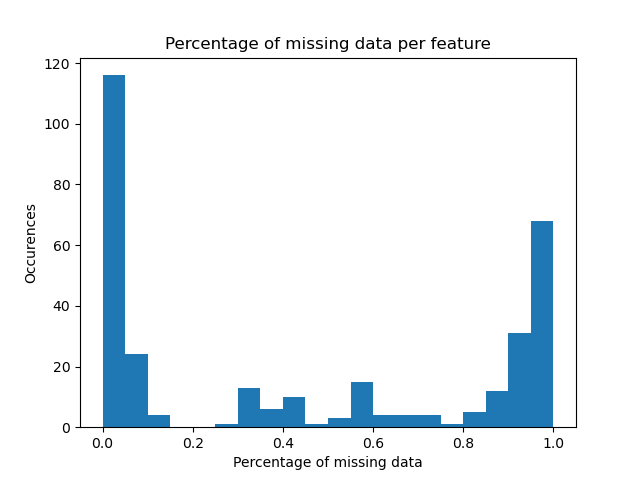
\includegraphics[width=0.4\textwidth]{Missing_data.png}  

    \caption{Percentage of missing data per feature}

    \label{fig:missing}  

\end{figure}



\vspace{0.5cm}

\noindent\begin{minipage}{\textwidth}
\centering
\begin{tabular}[c]{|l||l|l|l|l|}
  \hline
  Feature threshold & Outlier strategy & Fill method & F1 score (train) & F1 score (validation) \\
  \hline
  0.8 & smart & median & 0.4314 & 0.4360 [estimated]\\ 
  0.8 & smart & mode & 0.4309 & 0.4370 \\ 
  0.8 & aggressive & mode & 0.4293 [estimated] & 0.4350 [estimated] \\ 
  0.8 & std (threshold=5) & mode & 0.4305 & 0.4360 [estimated] \\ 
  0.8 & none & mode & 0.4229 [estimated] & 0.4210 [estimated] \\ 
  0.5 & smart & mode & 0.4298 & 0.4330 [estimated] \\ 
  \hline
\end{tabular}
\captionof{table}{Preprocessing Methods Comparison. This table shows the prediction accuracy of the Regularized Logistic Regression with different preprocessing strategies. Features threshold: percent of missing data in a feature above which it is removed. Outlier strategy: method to remove aberrant values in a feature (described above). Fill method: replace the NaN with either the mode or median of the column. Continuous features are normalized and categorical features are one-hot encoded in all presented cases.}
\label{tab:preprocessing_strategies}
\end{minipage}

\noindent\begin{minipage}{\textwidth}
\centering
\begin{tabular}[c]{|l||l|l|l|}
  \hline
  Model & F1 score (train) & F1 score (validation) & Parameters \\
  \hline
  MSE GD & 0.0101 & 0.0095 [estimated] & $\gamma=0.01$ \\ 
  MSE SGD & 0.1426 & 0.137 [AICrowd] & $\gamma=0.0046$ \\
  LSE & 0.4220 & 0.16 [AICrowd] & - \\
  Logistic & 0.4259 & 0.438 [AICrowd] & $\gamma=0.08$ \\
  Reg. Logistic & 0.4291 &  0.437 [AICrowd] & $\gamma=0.1$, $\lambda=10^{-6}$ \\
  Ridge & 0.0275 & 0.033 [AICrowd] & $\lambda=10^{-5}$ \\
  KNN & 0.3258 & 0.3181 [estimated] & $k=30$, factor$=9$ \\
  \hline
\end{tabular}
\captionof{table}{Models Comparison. This table shows a comparison of the different models accuracy for given (approximate best) parameters. Data was preprocessed with the method yielding overall best results (feature threshold at 0.8, "smart" outlier strategy, filling with the mode of the feature, normalizing continuous features and one-hot encoding categorical ones).}
\label{tab:models_comparison}
\end{minipage}

\vspace{0.3 cm}

\begin{figure}
    \centering
    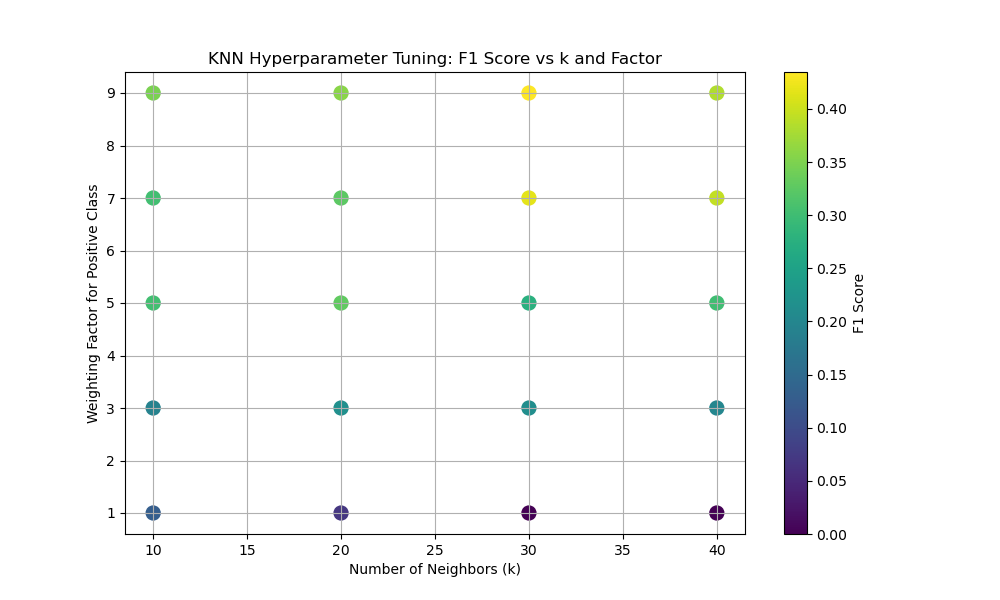
\includegraphics[width=0.4\textwidth]{KNN_F1_Scores_CV1.png}  

    \caption{KNN F1 score versus number of neighbors $k$ and the weighting factors for positive class.}

    \label{fig:KNN}  

\end{figure}



\end{document}

\bibliographystyle{IEEEtran}
\begin{thebibliography}{1}
\bibitem{brfss}
Centers for Disease Control and Prevention, ``Behavioral Risk Factor Surveillance System,'' 2015. [Online]. Available: https://www.cdc.gov/brfss/
\end{thebibliography}
